\documentclass{article}
\usepackage[utf8]{inputenc}

\usepackage{tikz}
\usetikzlibrary{positioning, fit}

\begin{document}

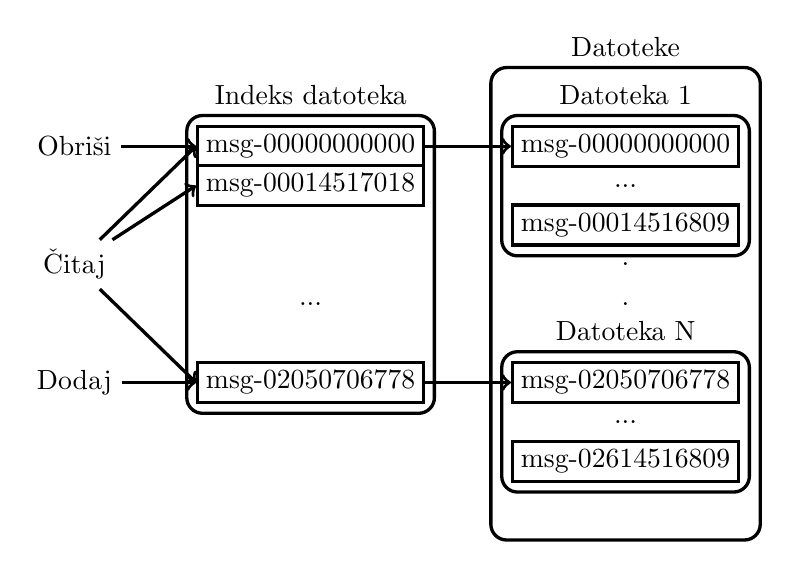
\begin{tikzpicture}[ % has a lot of options; consult the pgf manual
bend angle=45,
long_square/.style={rectangle, draw=black, fill=white, very thick, inner sep=3pt, minimum width=14mm},
rounded_square/.style={rectangle, rounded corners, draw=black, fill=white, very thick, inner sep=3pt, minimum width=14mm},
empty_circle/.style={rectangle, rounded corners=2mm, draw=black, fill=white, very thick, minimum size=4mm},
point/.style={circle, inner sep=0mm},
fit_square/.style={rectangle, rounded corners=2mm, draw=black, very thick},
both_arrow/.style={<->, very thick},
out_arrow/.style={->, very thick},
in_arrow/.style={<-, very thick},
above_edge_text/.style={above, midway, sloped}
]

\node[](delete) at (0,0) {Obriši};
\node[](read) at (0,-1.5) {Čitaj};
\node[](append) at (0,-3) {Dodaj};

\node[long_square](pointer_1) at (3,0) {msg-00000000000};
\node[long_square](pointer_2) at (3,-0.5) {msg-00014517018};
\node[](pointer_3) at (3,-1.5) {};
\node[](pointer_4) at (3,-2) {...};
\node[](pointer_5) at (3,-2.5) {};
\node[long_square](pointer_6) at (3,-3) {msg-02050706778};

\node[long_square](msg_1) at (7,0) {msg-00000000000};
\node[](msg_2) at (7,-0.5) {...};
\node[long_square](msg_3) at (7,-1) {msg-00014516809};

\node[](msg_4) at (7,-1.5) {.};
\node[](msg_5) at (7,-2) {.};

\node[long_square](msg_6) at (7,-3) {msg-02050706778};
\node[](msg_7) at (7,-3.5) {...};
\node[long_square](msg_8) at (7,-4) {msg-02614516809};

\node[fit_square, fit=(pointer_1) (pointer_2) (pointer_3) (pointer_4) (pointer_5) (pointer_6)] (index) {};
\node[anchor=south] at (index.north) {Indeks datoteka};

\node[fit_square, fit=(msg_1) (msg_2) (msg_3)] (file_1) {};
\node[anchor=south] at (file_1.north) {Datoteka 1};

\node[fit_square, fit=(msg_6) (msg_7) (msg_8)] (file_2) {};
\node[anchor=south] at (file_2.north) {Datoteka N};

\node[fit_square, minimum height=60mm, fit=(file_1) (file_2)] (files) {};
\node[anchor=south] at (files.north) {Datoteke};



\draw[out_arrow](delete) to [] node[auto]{} (pointer_1);
\draw[out_arrow](read) to [] node[auto]{} (pointer_1.west);
\draw[out_arrow](read) to [] node[auto]{} (pointer_2.west);
\draw[out_arrow](read) to [] node[auto]{} (pointer_6.west);
\draw[out_arrow](append) to [] node[auto]{} (pointer_6);

\draw[out_arrow](pointer_1) to [] node[auto]{} (msg_1);
\draw[out_arrow](pointer_6) to [] node[auto]{} (msg_6);

\end{tikzpicture}

\end{document}